\section{Verification}
\label{sec:verification}
This section describes the check of spatial and temporal order of accuracy using the Method of Manufactured Solutions in 2D and 3D for viscous and inviscid flows, characterization of stable time-step limits, assessment of computational cost per degree of freedom for a given error tolerance, and measurement of weak and strong scalability in GPUs and CPUs.

\subsection{Method of Manufactured Solutions}

\begin{figure}
\centering
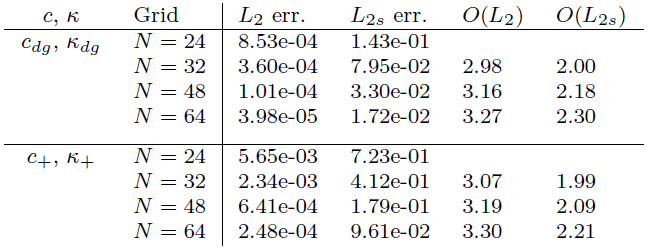
\includegraphics[height=35mm]{./figures/table_917} \\
\caption{Accuracy of ESFR schemes for flow generated by a time-dependent source term on triangular grids, for the case of $p = 2$. The inviscid and viscous numerical fluxes were computed using a Rusanov flux with $\lambda = 1$ and a LDG flux with $\tau = 0.1$ and $\beta = \pm 0.5n$.}
\label{fig:table_917}
\end{figure}

\begin{figure}
\centering
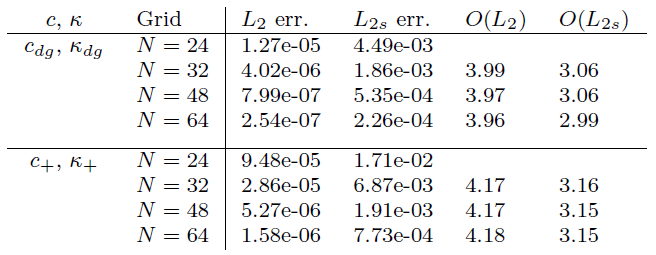
\includegraphics[height=35mm]{./figures/table_918} \\
\caption{Accuracy of ESFR schemes for flow generated by a time-dependent source term on triangular grids, for the case of $p = 3$. The inviscid and viscous numerical fluxes were computed using a Rusanov flux with $\lambda = 1$ and a LDG flux with $\tau = 0.1$ and $\beta = \pm 0.5n$.}
\label{fig:table_918}
\end{figure}

\begin{figure}
\centering
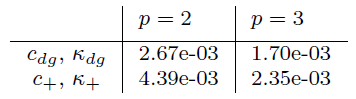
\includegraphics[height=20mm]{./figures/table_919} \\
\caption{Explicit time-step limits ($\Delta t_{max}$) of ESFR schemes for flow generated by a time-dependent source term on the triangular grid with $\tilde{N} = 48$, for the cases of $p = 2 and 3$. The inviscid and viscous numerical fluxes were computed using a Rusanov flux with $\lambda = 1$ and a LDG flux with $\tau = 0.1$ and $\beta = \pm 0.5n$.}
\label{fig:table_919}
\end{figure}

\begin{figure}
\centering
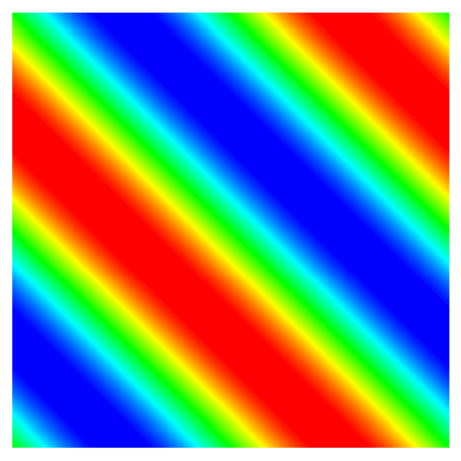
\includegraphics[height=60mm]{./figures/figure_912} \\
\caption{Contours of energy obtained using the ESFR scheme with $c = c_+$ and $\kappa = \kappa_+$ on the triangular grid with $\tilde{N} = 32$ for the case of $p = 3$. The inviscid and viscous numerical fluxes were computed using a Rusanov flux with $\lambda = 1$ and a LDG flux with $\tau = 0.1$ and $\beta = \pm 0.5n$.}
\label{fig:figure_912}
\end{figure}

\begin{figure}
\centering
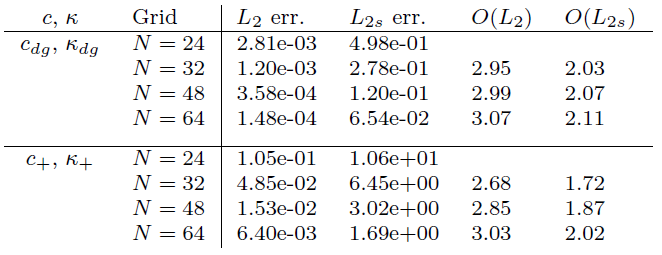
\includegraphics[height=35mm]{./figures/table_920} \\
\caption{Accuracy of ESFR schemes for flow generated by a time-dependent source term on tetrahedral grids, for the case of $p = 2$. The inviscid and viscous numerical fluxes were computed using a Rusanov flux with $\lambda = 1$ and a LDG flux with $\tau = 0.1$ and $\beta = \pm 0.5n$.}
\label{fig:table_920}
\end{figure}

\begin{figure}
\centering
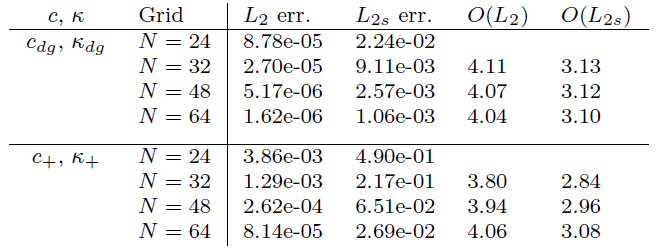
\includegraphics[height=30mm]{./figures/table_921} \\
\caption{Accuracy of ESFR schemes for flow generated by a time-dependent source term on tetrahedral grids, for the case of $p = 3$. The inviscid and viscous numerical fluxes were computed using a Rusanov flux with $\lambda = 1$ and a LDG flux with $\tau = 0.1$ and $\beta = \pm 0.5n$.}
\label{fig:table_921}
\end{figure}

\begin{figure}
\centering
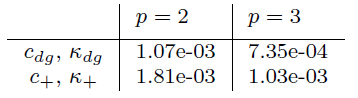
\includegraphics[height=15mm]{./figures/table_922} \\
\caption{Explicit time-step limits ($\Delta t_{max}$) of ESFR schemes for flow generated by a time-dependent source term on the triangular grid with $\tilde{N} = 48$, for the cases of $p = 2 and 3$. The inviscid and viscous numerical fluxes were computed using a Rusanov flux with $\lambda = 1$ and a LDG flux with $\tau = 0.1$ and $\beta = \pm 0.5n$.}
\label{fig:table_922}
\end{figure}

\newpage
\begin{figure}
\centering
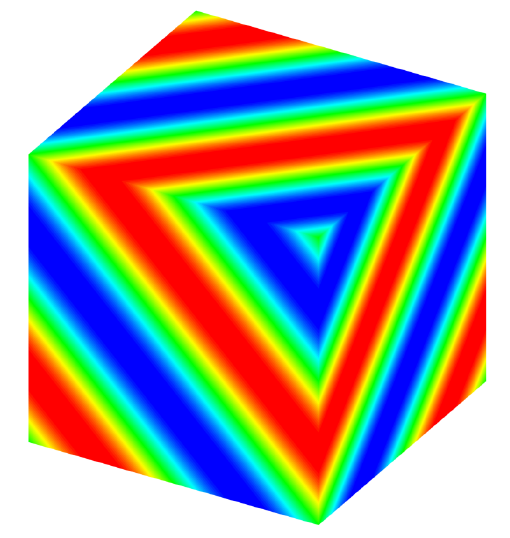
\includegraphics[height=60mm]{./figures/figure_913} \\
\caption{Contours of energy obtained using the ESFR scheme with $c = c_+$ and $\kappa = \kappa_+$ on the tetrahedral grid with $\tilde{N} = 32$ for the case of $p = 3$. The inviscid and viscous numerical fluxes were computed using a Rusanov flux with $\lambda = 1$ and a LDG flux with $\tau = 0.1$ and $\beta = \pm 0.5n$.}
\label{fig:figure_913}
\end{figure}
%\subsection{Time Stepping Order of Accuracy and limits}
%Generate highly refined grid and advance in time with progressively smaller time-steps. Calculate the error and find the order of the truncation error.
%
%\subsection{Efficiency}
%Description of the number of calculations performed per time-step, the time each time-step takes, the Teraflops achieved in each test-case mentioned here.
%
%
%\subsection{Weak and Strong Scalability}
%Full study in \cite{castonguay2011}.